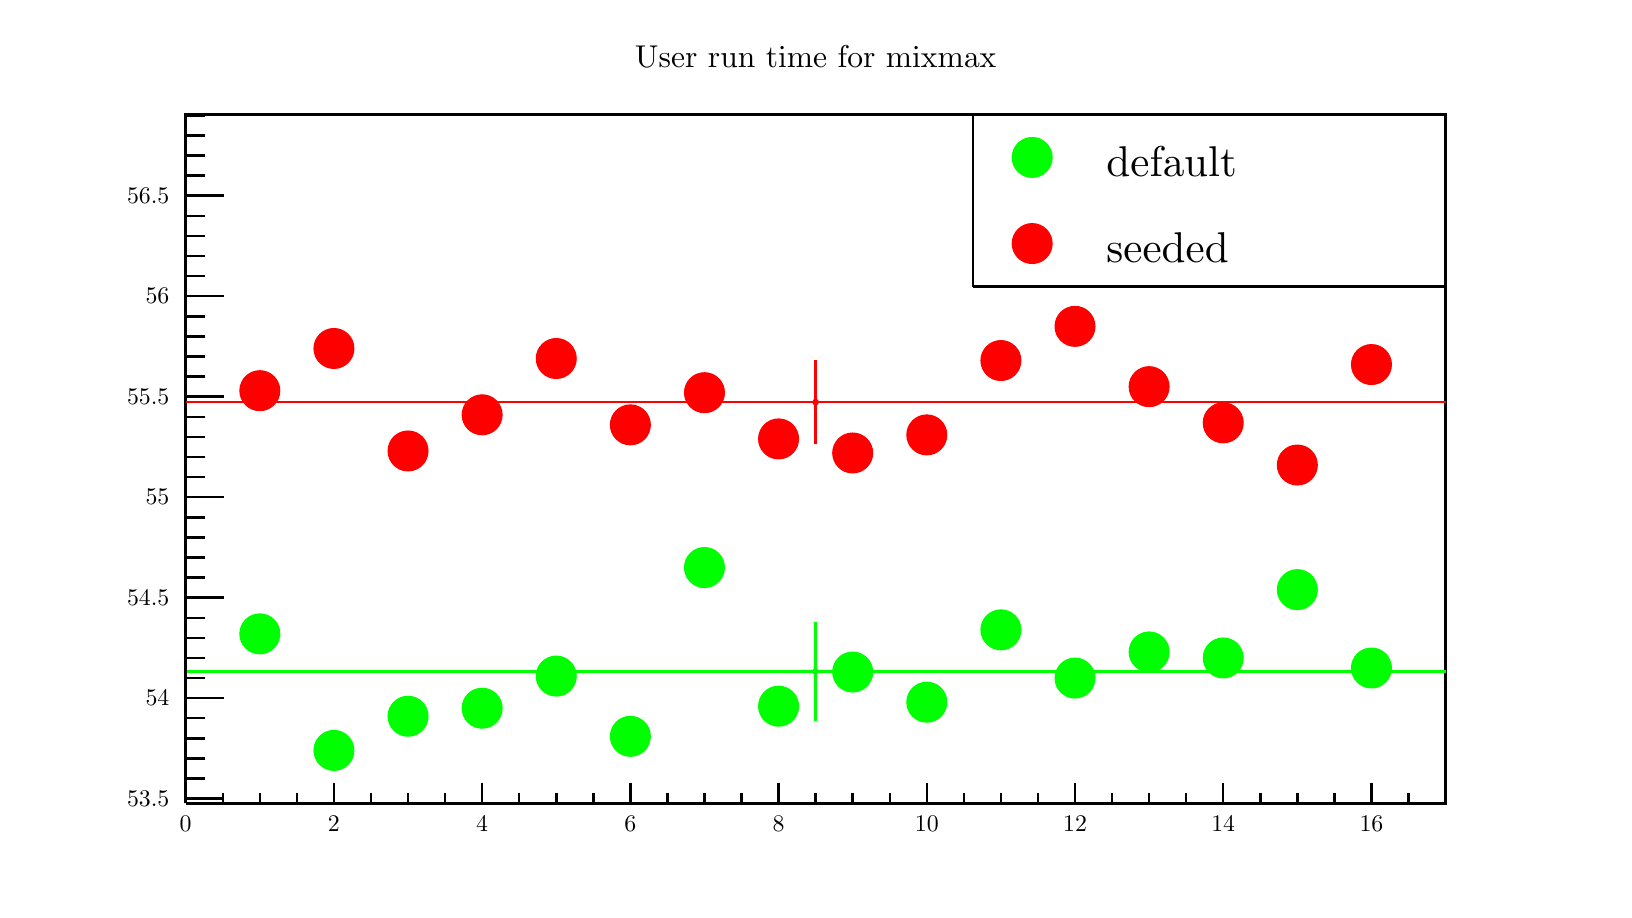
\begin{tikzpicture}
\pgfdeclareplotmark{cross} {
\pgfpathmoveto{\pgfpoint{-0.3\pgfplotmarksize}{\pgfplotmarksize}}
\pgfpathlineto{\pgfpoint{+0.3\pgfplotmarksize}{\pgfplotmarksize}}
\pgfpathlineto{\pgfpoint{+0.3\pgfplotmarksize}{0.3\pgfplotmarksize}}
\pgfpathlineto{\pgfpoint{+1\pgfplotmarksize}{0.3\pgfplotmarksize}}
\pgfpathlineto{\pgfpoint{+1\pgfplotmarksize}{-0.3\pgfplotmarksize}}
\pgfpathlineto{\pgfpoint{+0.3\pgfplotmarksize}{-0.3\pgfplotmarksize}}
\pgfpathlineto{\pgfpoint{+0.3\pgfplotmarksize}{-1.\pgfplotmarksize}}
\pgfpathlineto{\pgfpoint{-0.3\pgfplotmarksize}{-1.\pgfplotmarksize}}
\pgfpathlineto{\pgfpoint{-0.3\pgfplotmarksize}{-0.3\pgfplotmarksize}}
\pgfpathlineto{\pgfpoint{-1.\pgfplotmarksize}{-0.3\pgfplotmarksize}}
\pgfpathlineto{\pgfpoint{-1.\pgfplotmarksize}{0.3\pgfplotmarksize}}
\pgfpathlineto{\pgfpoint{-0.3\pgfplotmarksize}{0.3\pgfplotmarksize}}
\pgfpathclose
\pgfusepathqstroke
}
\pgfdeclareplotmark{cross*} {
\pgfpathmoveto{\pgfpoint{-0.3\pgfplotmarksize}{\pgfplotmarksize}}
\pgfpathlineto{\pgfpoint{+0.3\pgfplotmarksize}{\pgfplotmarksize}}
\pgfpathlineto{\pgfpoint{+0.3\pgfplotmarksize}{0.3\pgfplotmarksize}}
\pgfpathlineto{\pgfpoint{+1\pgfplotmarksize}{0.3\pgfplotmarksize}}
\pgfpathlineto{\pgfpoint{+1\pgfplotmarksize}{-0.3\pgfplotmarksize}}
\pgfpathlineto{\pgfpoint{+0.3\pgfplotmarksize}{-0.3\pgfplotmarksize}}
\pgfpathlineto{\pgfpoint{+0.3\pgfplotmarksize}{-1.\pgfplotmarksize}}
\pgfpathlineto{\pgfpoint{-0.3\pgfplotmarksize}{-1.\pgfplotmarksize}}
\pgfpathlineto{\pgfpoint{-0.3\pgfplotmarksize}{-0.3\pgfplotmarksize}}
\pgfpathlineto{\pgfpoint{-1.\pgfplotmarksize}{-0.3\pgfplotmarksize}}
\pgfpathlineto{\pgfpoint{-1.\pgfplotmarksize}{0.3\pgfplotmarksize}}
\pgfpathlineto{\pgfpoint{-0.3\pgfplotmarksize}{0.3\pgfplotmarksize}}
\pgfpathclose
\pgfusepathqfillstroke
}
\pgfdeclareplotmark{newstar} {
\pgfpathmoveto{\pgfqpoint{0pt}{\pgfplotmarksize}}
\pgfpathlineto{\pgfqpointpolar{44}{0.5\pgfplotmarksize}}
\pgfpathlineto{\pgfqpointpolar{18}{\pgfplotmarksize}}
\pgfpathlineto{\pgfqpointpolar{-20}{0.5\pgfplotmarksize}}
\pgfpathlineto{\pgfqpointpolar{-54}{\pgfplotmarksize}}
\pgfpathlineto{\pgfqpointpolar{-90}{0.5\pgfplotmarksize}}
\pgfpathlineto{\pgfqpointpolar{234}{\pgfplotmarksize}}
\pgfpathlineto{\pgfqpointpolar{198}{0.5\pgfplotmarksize}}
\pgfpathlineto{\pgfqpointpolar{162}{\pgfplotmarksize}}
\pgfpathlineto{\pgfqpointpolar{134}{0.5\pgfplotmarksize}}
\pgfpathclose
\pgfusepathqstroke
}
\pgfdeclareplotmark{newstar*} {
\pgfpathmoveto{\pgfqpoint{0pt}{\pgfplotmarksize}}
\pgfpathlineto{\pgfqpointpolar{44}{0.5\pgfplotmarksize}}
\pgfpathlineto{\pgfqpointpolar{18}{\pgfplotmarksize}}
\pgfpathlineto{\pgfqpointpolar{-20}{0.5\pgfplotmarksize}}
\pgfpathlineto{\pgfqpointpolar{-54}{\pgfplotmarksize}}
\pgfpathlineto{\pgfqpointpolar{-90}{0.5\pgfplotmarksize}}
\pgfpathlineto{\pgfqpointpolar{234}{\pgfplotmarksize}}
\pgfpathlineto{\pgfqpointpolar{198}{0.5\pgfplotmarksize}}
\pgfpathlineto{\pgfqpointpolar{162}{\pgfplotmarksize}}
\pgfpathlineto{\pgfqpointpolar{134}{0.5\pgfplotmarksize}}
\pgfpathclose
\pgfusepathqfillstroke
}
\definecolor{c}{rgb}{1,1,1};
\draw [color=c, fill=c] (0,0) rectangle (20,10.9387);
\draw [color=c, fill=c] (2,1.09387) rectangle (18,9.84481);
\definecolor{c}{rgb}{0,0,0};
\draw [c,line width=0.9] (2,1.09387) -- (2,9.84481) -- (18,9.84481) -- (18,1.09387) -- (2,1.09387);
\definecolor{c}{rgb}{1,1,1};
\draw [color=c, fill=c] (2,1.09387) rectangle (18,9.84481);
\definecolor{c}{rgb}{0,0,0};
\draw [c,line width=0.9] (2,1.09387) -- (2,9.84481) -- (18,9.84481) -- (18,1.09387) -- (2,1.09387);
\definecolor{c}{rgb}{0,1,0};
\draw [c,line width=0.9] (10,2.13604) -- (10,2.76876);
\draw [c,line width=0.9] (10,2.76876) -- (10,3.40149);
\draw [c,line width=0.9] (2,2.76876) -- (10,2.76876);
\draw [c,line width=0.9] (10,2.76876) -- (18,2.76876);
\foreach \P in {(10,2.76876)}{\draw[mark options={color=c,fill=c},mark size=2.402402pt,mark=*,mark size=1pt] plot coordinates {\P};}
\definecolor{c}{rgb}{0,0,0};
\draw [c,line width=0.9] (2,1.09387) -- (18,1.09387);
\draw [c,line width=0.9] (2,1.3564) -- (2,1.09387);
\draw [c,line width=0.9] (2.47059,1.22513) -- (2.47059,1.09387);
\draw [c,line width=0.9] (2.94118,1.22513) -- (2.94118,1.09387);
\draw [c,line width=0.9] (3.41176,1.22513) -- (3.41176,1.09387);
\draw [c,line width=0.9] (3.88235,1.3564) -- (3.88235,1.09387);
\draw [c,line width=0.9] (4.35294,1.22513) -- (4.35294,1.09387);
\draw [c,line width=0.9] (4.82353,1.22513) -- (4.82353,1.09387);
\draw [c,line width=0.9] (5.29412,1.22513) -- (5.29412,1.09387);
\draw [c,line width=0.9] (5.76471,1.3564) -- (5.76471,1.09387);
\draw [c,line width=0.9] (6.23529,1.22513) -- (6.23529,1.09387);
\draw [c,line width=0.9] (6.70588,1.22513) -- (6.70588,1.09387);
\draw [c,line width=0.9] (7.17647,1.22513) -- (7.17647,1.09387);
\draw [c,line width=0.9] (7.64706,1.3564) -- (7.64706,1.09387);
\draw [c,line width=0.9] (8.11765,1.22513) -- (8.11765,1.09387);
\draw [c,line width=0.9] (8.58823,1.22513) -- (8.58823,1.09387);
\draw [c,line width=0.9] (9.05882,1.22513) -- (9.05882,1.09387);
\draw [c,line width=0.9] (9.52941,1.3564) -- (9.52941,1.09387);
\draw [c,line width=0.9] (10,1.22513) -- (10,1.09387);
\draw [c,line width=0.9] (10.4706,1.22513) -- (10.4706,1.09387);
\draw [c,line width=0.9] (10.9412,1.22513) -- (10.9412,1.09387);
\draw [c,line width=0.9] (11.4118,1.3564) -- (11.4118,1.09387);
\draw [c,line width=0.9] (11.8824,1.22513) -- (11.8824,1.09387);
\draw [c,line width=0.9] (12.3529,1.22513) -- (12.3529,1.09387);
\draw [c,line width=0.9] (12.8235,1.22513) -- (12.8235,1.09387);
\draw [c,line width=0.9] (13.2941,1.3564) -- (13.2941,1.09387);
\draw [c,line width=0.9] (13.7647,1.22513) -- (13.7647,1.09387);
\draw [c,line width=0.9] (14.2353,1.22513) -- (14.2353,1.09387);
\draw [c,line width=0.9] (14.7059,1.22513) -- (14.7059,1.09387);
\draw [c,line width=0.9] (15.1765,1.3564) -- (15.1765,1.09387);
\draw [c,line width=0.9] (15.6471,1.22513) -- (15.6471,1.09387);
\draw [c,line width=0.9] (16.1176,1.22513) -- (16.1176,1.09387);
\draw [c,line width=0.9] (16.5882,1.22513) -- (16.5882,1.09387);
\draw [c,line width=0.9] (17.0588,1.3564) -- (17.0588,1.09387);
\draw [c,line width=0.9] (17.0588,1.3564) -- (17.0588,1.09387);
\draw [c,line width=0.9] (17.5294,1.22513) -- (17.5294,1.09387);
\draw [c,line width=0.9] (18,1.22513) -- (18,1.09387);
\draw [anchor=base] (2,0.732891) node[scale=0.861703, color=c, rotate=0]{0};
\draw [anchor=base] (3.88235,0.732891) node[scale=0.861703, color=c, rotate=0]{2};
\draw [anchor=base] (5.76471,0.732891) node[scale=0.861703, color=c, rotate=0]{4};
\draw [anchor=base] (7.64706,0.732891) node[scale=0.861703, color=c, rotate=0]{6};
\draw [anchor=base] (9.52941,0.732891) node[scale=0.861703, color=c, rotate=0]{8};
\draw [anchor=base] (11.4118,0.732891) node[scale=0.861703, color=c, rotate=0]{10};
\draw [anchor=base] (13.2941,0.732891) node[scale=0.861703, color=c, rotate=0]{12};
\draw [anchor=base] (15.1765,0.732891) node[scale=0.861703, color=c, rotate=0]{14};
\draw [anchor=base] (17.0588,0.732891) node[scale=0.861703, color=c, rotate=0]{16};
\draw [c,line width=0.9] (2,1.09387) -- (2,9.84481);
\draw [c,line width=0.9] (2.48,1.15448) -- (2,1.15448);
\draw [c,line width=0.9] (2.24,1.40971) -- (2,1.40971);
\draw [c,line width=0.9] (2.24,1.66493) -- (2,1.66493);
\draw [c,line width=0.9] (2.24,1.92015) -- (2,1.92015);
\draw [c,line width=0.9] (2.24,2.17537) -- (2,2.17537);
\draw [c,line width=0.9] (2.48,2.43059) -- (2,2.43059);
\draw [c,line width=0.9] (2.24,2.68582) -- (2,2.68582);
\draw [c,line width=0.9] (2.24,2.94104) -- (2,2.94104);
\draw [c,line width=0.9] (2.24,3.19626) -- (2,3.19626);
\draw [c,line width=0.9] (2.24,3.45148) -- (2,3.45148);
\draw [c,line width=0.9] (2.48,3.70671) -- (2,3.70671);
\draw [c,line width=0.9] (2.24,3.96193) -- (2,3.96193);
\draw [c,line width=0.9] (2.24,4.21715) -- (2,4.21715);
\draw [c,line width=0.9] (2.24,4.47237) -- (2,4.47237);
\draw [c,line width=0.9] (2.24,4.7276) -- (2,4.7276);
\draw [c,line width=0.9] (2.48,4.98282) -- (2,4.98282);
\draw [c,line width=0.9] (2.24,5.23804) -- (2,5.23804);
\draw [c,line width=0.9] (2.24,5.49326) -- (2,5.49326);
\draw [c,line width=0.9] (2.24,5.74849) -- (2,5.74849);
\draw [c,line width=0.9] (2.24,6.00371) -- (2,6.00371);
\draw [c,line width=0.9] (2.48,6.25893) -- (2,6.25893);
\draw [c,line width=0.9] (2.24,6.51415) -- (2,6.51415);
\draw [c,line width=0.9] (2.24,6.76938) -- (2,6.76938);
\draw [c,line width=0.9] (2.24,7.0246) -- (2,7.0246);
\draw [c,line width=0.9] (2.24,7.27982) -- (2,7.27982);
\draw [c,line width=0.9] (2.48,7.53504) -- (2,7.53504);
\draw [c,line width=0.9] (2.24,7.79027) -- (2,7.79027);
\draw [c,line width=0.9] (2.24,8.04549) -- (2,8.04549);
\draw [c,line width=0.9] (2.24,8.30071) -- (2,8.30071);
\draw [c,line width=0.9] (2.24,8.55593) -- (2,8.55593);
\draw [c,line width=0.9] (2.48,8.81116) -- (2,8.81116);
\draw [c,line width=0.9] (2.48,1.15448) -- (2,1.15448);
\draw [c,line width=0.9] (2.48,8.81116) -- (2,8.81116);
\draw [c,line width=0.9] (2.24,9.06638) -- (2,9.06638);
\draw [c,line width=0.9] (2.24,9.3216) -- (2,9.3216);
\draw [c,line width=0.9] (2.24,9.57682) -- (2,9.57682);
\draw [c,line width=0.9] (2.24,9.83204) -- (2,9.83204);
\draw [anchor= east] (1.9,1.15448) node[scale=0.861703, color=c, rotate=0]{53.5};
\draw [anchor= east] (1.9,2.43059) node[scale=0.861703, color=c, rotate=0]{54};
\draw [anchor= east] (1.9,3.70671) node[scale=0.861703, color=c, rotate=0]{54.5};
\draw [anchor= east] (1.9,4.98282) node[scale=0.861703, color=c, rotate=0]{55};
\draw [anchor= east] (1.9,6.25893) node[scale=0.861703, color=c, rotate=0]{55.5};
\draw [anchor= east] (1.9,7.53504) node[scale=0.861703, color=c, rotate=0]{56};
\draw [anchor= east] (1.9,8.81116) node[scale=0.861703, color=c, rotate=0]{56.5};
\definecolor{c}{rgb}{1,0,0};
\draw [c,line width=0.9] (10,5.65574) -- (10,6.19034);
\draw [c,line width=0.9] (10,6.19034) -- (10,6.72495);
\draw [c,line width=0.9] (2,6.19034) -- (10,6.19034);
\draw [c,line width=0.9] (10,6.19034) -- (18,6.19034);
\foreach \P in {(10,6.19034)}{\draw[mark options={color=c,fill=c},mark size=2.402402pt,mark=*,mark size=1pt] plot coordinates {\P};}
\definecolor{c}{rgb}{0,1,0};
\foreach \P in {(2.94118,3.24731), (3.88235,1.76702), (4.82353,2.20089), (5.76471,2.30298), (6.70588,2.71134), (7.64706,1.94567), (8.58823,4.08954), (9.52941,2.32851), (10.4706,2.76238), (11.4118,2.37955), (12.3529,3.29835), (13.2941,2.68582),
 (14.2353,3.01761), (15.1765,2.94104), (16.1176,3.8088), (17.0588,2.81343)}{\draw[mark options={color=c,fill=c},mark size=7.207207pt,mark=*] plot coordinates {\P};}
\definecolor{c}{rgb}{1,0,0};
\foreach \P in {(2.94118,6.3355), (3.88235,6.87146), (4.82353,5.56983), (5.76471,6.02923), (6.70588,6.74385), (7.64706,5.90162), (8.58823,6.30998), (9.52941,5.72296), (10.4706,5.54431), (11.4118,5.77401), (12.3529,6.71833), (13.2941,7.15221),
 (14.2353,6.38654), (15.1765,5.92714), (16.1176,5.39117), (17.0588,6.66729)}{\draw[mark options={color=c,fill=c},mark size=7.207207pt,mark=*] plot coordinates {\P};}
\definecolor{c}{rgb}{1,1,1};
\draw [color=c, fill=c] (12,7.65707) rectangle (18,9.84481);
\definecolor{c}{rgb}{0,0,0};
\draw [c,line width=0.9] (12,7.65707) -- (18,7.65707);
\draw [c,line width=0.9] (18,7.65707) -- (18,9.84481);
\draw [c,line width=0.9] (18,9.84481) -- (12,9.84481);
\draw [c,line width=0.9] (12,9.84481) -- (12,7.65707);
\draw [anchor=base west] (13.5,9.05175) node[scale=1.55662, color=c, rotate=0]{default};
\definecolor{c}{rgb}{1,1,1};
\draw [c] (12.225,8.91502) -- (13.275,8.91502) -- (13.275,9.68073) -- (12.225,9.68073);
\draw [c,line width=0.9] (12.225,9.29787) -- (13.275,9.29787);
\definecolor{c}{rgb}{0,1,0};
\foreach \P in {(12.75,9.29787)}{\draw[mark options={color=c,fill=c},mark size=7.207207pt,mark=*] plot coordinates {\P};}
\definecolor{c}{rgb}{0,0,0};
\draw [anchor=base west] (13.5,7.95788) node[scale=1.55662, color=c, rotate=0]{seeded};
\definecolor{c}{rgb}{1,1,1};
\draw [c] (12.225,7.82115) -- (13.275,7.82115) -- (13.275,8.58686) -- (12.225,8.58686);
\draw [c,line width=0.9] (12.225,8.20401) -- (13.275,8.20401);
\definecolor{c}{rgb}{1,0,0};
\foreach \P in {(12.75,8.20401)}{\draw[mark options={color=c,fill=c},mark size=7.207207pt,mark=*] plot coordinates {\P};}
\definecolor{c}{rgb}{0,0,0};
\draw (10,10.5832) node[scale=1.13967, color=c, rotate=0]{User run time for mixmax};
\end{tikzpicture}
